
\documentclass[11pt]{article}
\usepackage[margin=1in]{geometry}
\usepackage{graphicx}
\usepackage{booktabs}
\usepackage{array}
\usepackage{float}
\usepackage{hyperref}
\usepackage{siunitx}
\usepackage{caption}
\usepackage{xcolor}
\usepackage{enumitem}
\usepackage{longtable}

\hypersetup{
    colorlinks=true,
    linkcolor=blue,
    urlcolor=blue
}

\title{Comparison of AdamW and Muon for LoRA Fine-Tuning of Qwen2.5-0.5B}
\author{Danil Eremenko}
\date{March 2026}

\begin{document}
\maketitle

\begin{abstract}
This report compares AdamW and Muon for LoRA fine-tuning of Qwen2.5-0.5B on a consumer AMD GPU.
The experiments use a matched setup with 5,000 training samples from OpenWebText-100k, sequence length 512, batch size 4, and 2 epochs.
We evaluate the optimizers by convergence proxy, wall-clock time, peak GPU memory, optimizer-step overhead, and downstream quality on PIQA.
In the tuned matched runs, AdamW and Muon reached very similar final training losses, but AdamW was substantially faster while using essentially the same peak memory.
PIQA results were nearly identical for the two fine-tuned models and slightly below the unfine-tuned base model, suggesting that short generic-text fine-tuning did not improve a commonsense QA benchmark in this setting.
\end{abstract}

\section{Introduction}
Optimizer choice affects both training dynamics and practical efficiency.
The task for this project is to compare recent optimization strategies for Qwen2.5-0.5B LoRA fine-tuning using training time, maximum memory usage, final model quality, and convergence as the main criteria.
The required training data source is at least 1\% of OpenWebText-100k, and the evaluation benchmark is PIQA.
The baseline optimizers required by the task are AdamW and Muon.

The present work focuses on a reproducible base-task comparison between AdamW and Muon on a single AMD Radeon RX 7900 XTX GPU under ROCm.
Challenge extensions such as MeZO and deliberate Muon+AdamW hybrid training are left for follow-up work.

\section{Experimental Setup}
\subsection{Hardware and software}
Experiments were run on an AMD Radeon RX 7900 XTX with ROCm-enabled PyTorch.
The training code uses Hugging Face Transformers and PEFT, but the training loop itself is implemented manually rather than through an orchestration framework such as Accelerate, in order to keep timing and memory measurements explicit.

\subsection{Model and adaptation setup}
The base model is Qwen2.5-0.5B.
LoRA was applied to the \texttt{q\_proj} and \texttt{v\_proj} modules with rank $r=8$, $\alpha=16$, and dropout 0.1.
Only LoRA adapter weights were trainable.

A parameter routing inspection showed that the Muon branch received 96 trainable tensors totaling 540,672 elements, while the auxiliary Adam branch received zero trainable parameters.
Therefore, although the code path used a Muon wrapper capable of handling an Adam side branch, the actual Muon experiments in this report were effectively pure Muon on the trainable LoRA weights.

\subsection{Training data and workload}
All main experiments used the same workload:
\begin{itemize}[leftmargin=1.5em]
    \item 5,000 samples from \texttt{Elriggs/openwebtext-100k}
    \item sequence length 512
    \item micro-batch size 4
    \item gradient accumulation 1
    \item effective batch size 4
    \item 2 epochs
    \item seed 42
\end{itemize}

A learning-rate sweep was performed separately for AdamW and Muon:
\begin{itemize}[leftmargin=1.5em]
    \item AdamW: $10^{-4}$, $3 \cdot 10^{-4}$, $10^{-3}$, $3 \cdot 10^{-3}$
    \item Muon: $3 \cdot 10^{-4}$, $10^{-3}$, $3 \cdot 10^{-3}$, $10^{-2}$
\end{itemize}

\subsection{Metrics}
For each run, the following quantities were recorded:
\begin{itemize}[leftmargin=1.5em]
    \item total training time
    \item peak GPU memory
    \item average loss over the last 10 logged points
    \item final logged loss
    \item average per-step time
    \item average optimizer-step time
\end{itemize}

For downstream quality, the best tuned AdamW and Muon checkpoints were evaluated on PIQA with \texttt{lm-evaluation-harness}.
The unfine-tuned base model was also evaluated as a reference point.

\section{Results}
\subsection{Learning-rate sweep}
Figure~\ref{fig:lr-loss} shows the average loss over the last ten logged points across the learning-rate sweep.
For both optimizers, the best result was obtained at a learning rate of $10^{-3}$.
Muon degraded sharply at $10^{-2}$, while AdamW was comparatively stable across the tested range.

\begin{figure}[H]
    \centering
    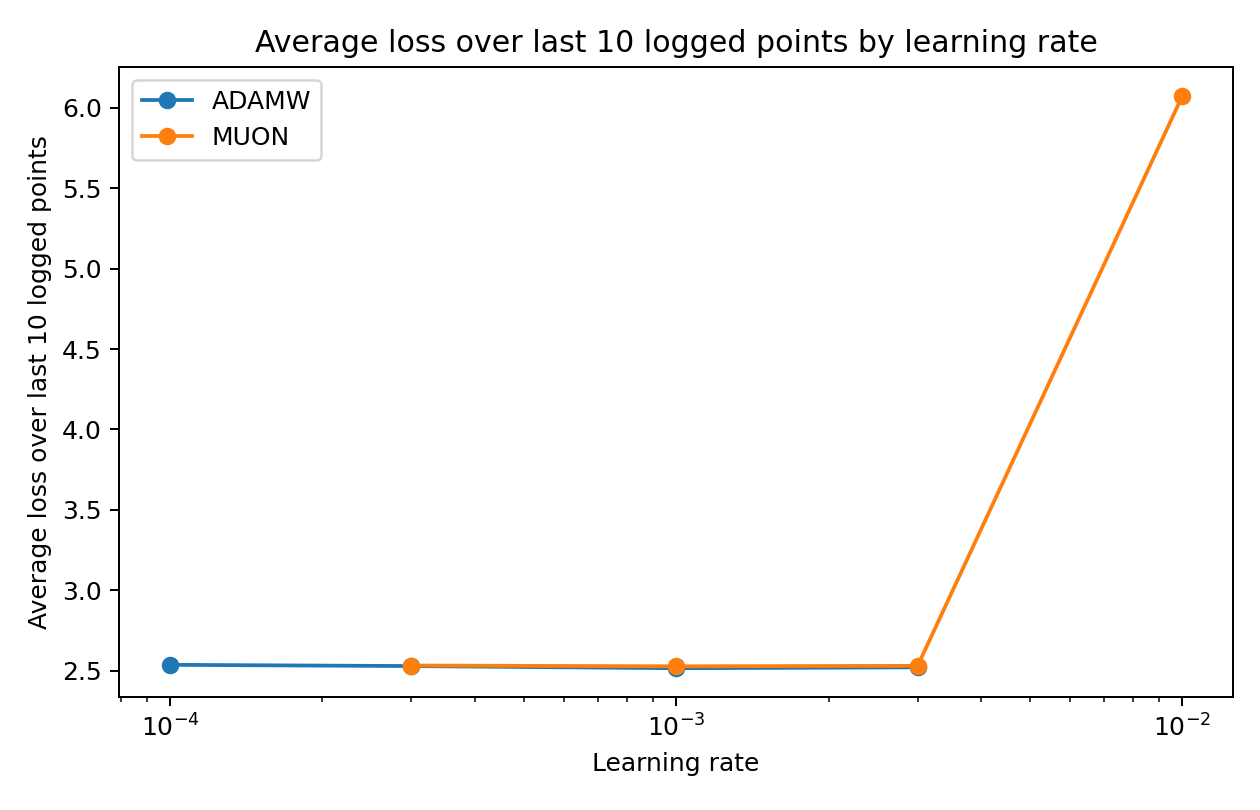
\includegraphics[width=0.78\textwidth]{figures/lr_vs_tail_loss.png}
    \caption{Average loss over the last 10 logged points as a function of learning rate.}
    \label{fig:lr-loss}
\end{figure}

Figure~\ref{fig:lr-time} shows that AdamW remained faster than Muon across the sweep.
The wall-clock gap is modest at the full-run level but consistent.

\begin{figure}[H]
    \centering
    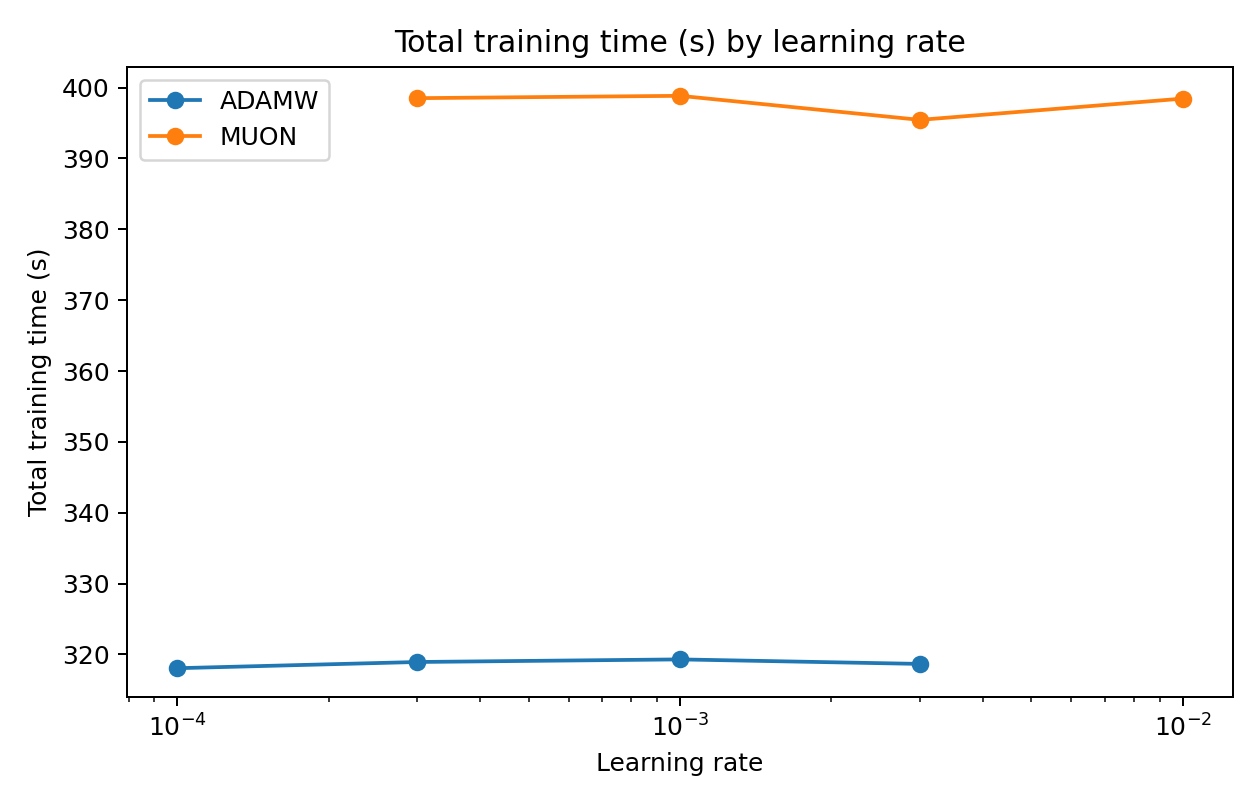
\includegraphics[width=0.78\textwidth]{figures/lr_vs_time.png}
    \caption{Total training time as a function of learning rate.}
    \label{fig:lr-time}
\end{figure}

\subsection{Best matched comparison}
Table~\ref{tab:main-comp} reports the best run for each optimizer under the matched workload.
AdamW and Muon reached very similar training losses, with AdamW slightly lower on both the final logged loss and the average over the last ten logged points.
The main practical difference is runtime: AdamW finished about 79.5 seconds faster.
Peak memory was effectively identical.

\begin{table}[H]
\centering
\caption{Best tuned matched runs (5,000 samples, 2 epochs, sequence length 512, batch size 4).}
\label{tab:main-comp}
\begin{tabular}{lrrrrrr}
\toprule
Optimizer & LR & Time (s) & Peak mem (GB) & Final loss & Avg. last 10 & Avg. opt. step (s) \\
\midrule
AdamW & 0.001 & 319.31 & 7.546 & 2.496 & 2.517 & 0.0009 \\
Muon  & 0.001 & 398.84 & 7.544 & 2.503 & 2.529 & 0.0293 \\
\bottomrule
\end{tabular}
\end{table}

The optimizer-step overhead is visualized in Figure~\ref{fig:opt-overhead}.
Muon's average optimizer-step time is much larger than AdamW's, which explains why it does not translate into a wall-clock advantage here.

\begin{figure}[H]
    \centering
    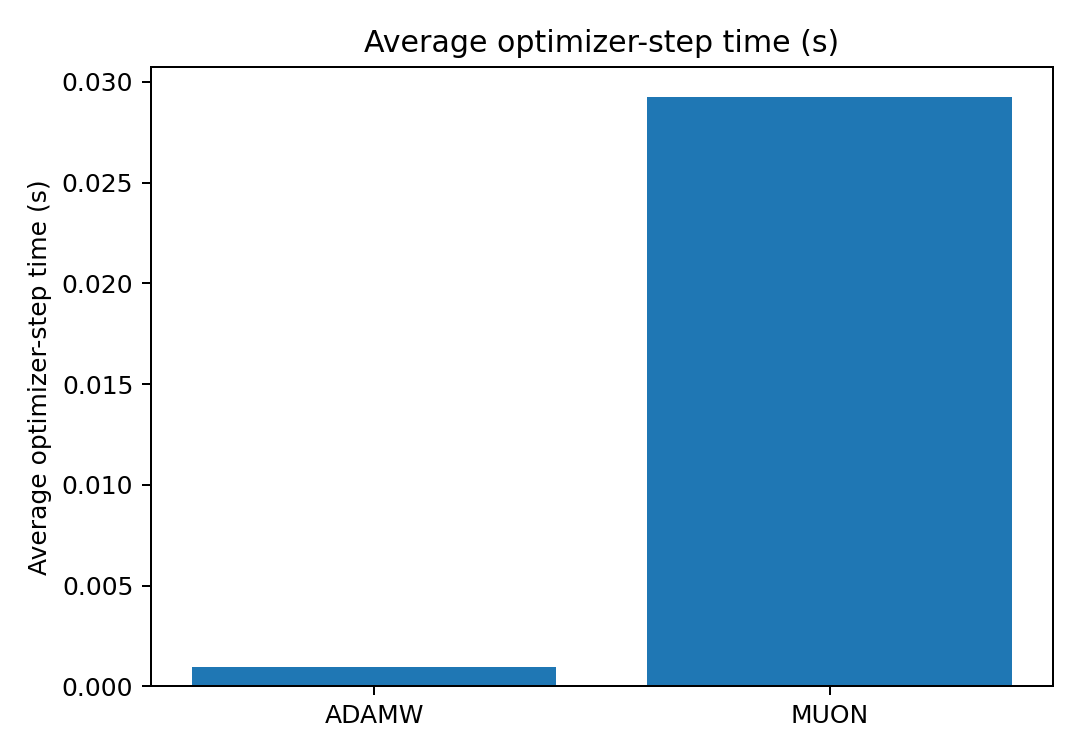
\includegraphics[width=0.62\textwidth]{figures/best_optimizer_overhead.png}
    \caption{Average optimizer-step time for the best matched runs.}
    \label{fig:opt-overhead}
\end{figure}

Figures~\ref{fig:best-time}, \ref{fig:best-mem}, and \ref{fig:best-loss} summarize the main matched comparison.

\begin{figure}[H]
    \centering
    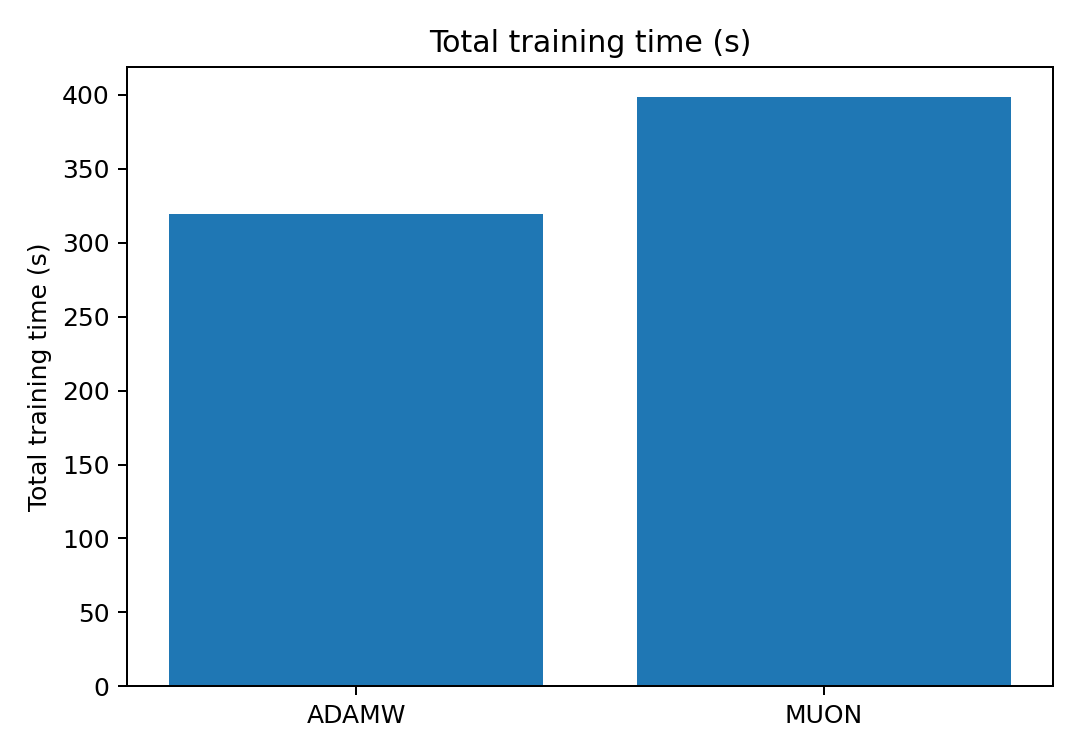
\includegraphics[width=0.58\textwidth]{figures/best_time_comparison.png}
    \caption{Total training time for the best matched runs.}
    \label{fig:best-time}
\end{figure}

\begin{figure}[H]
    \centering
    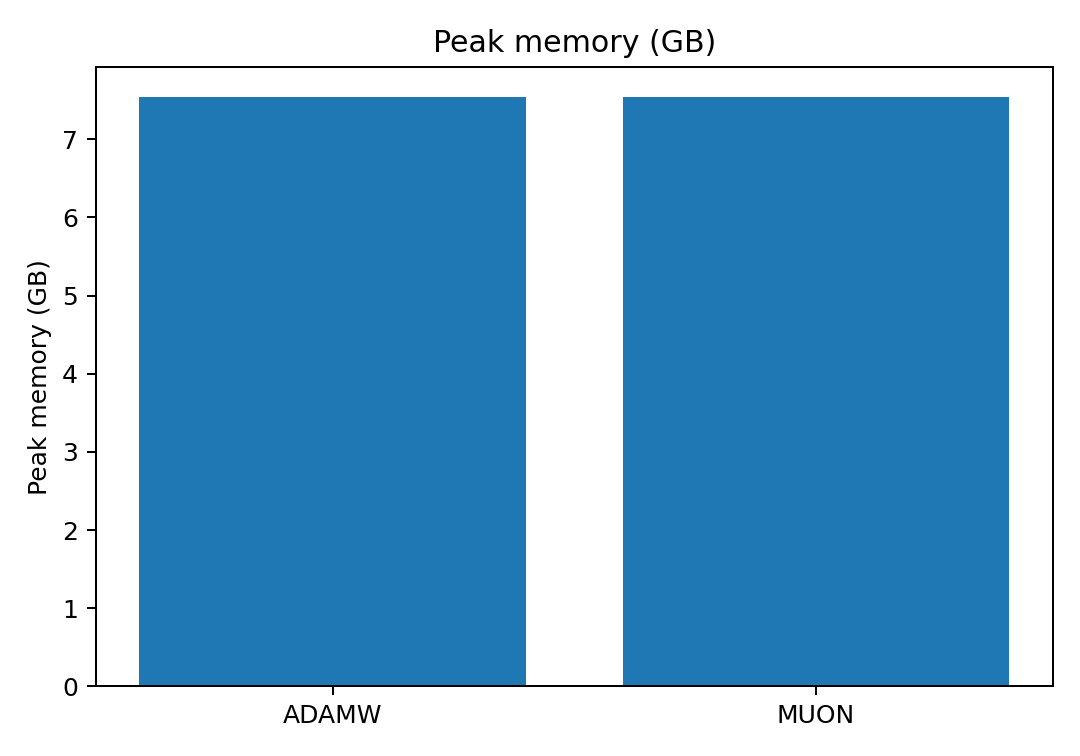
\includegraphics[width=0.58\textwidth]{figures/best_memory_comparison.png}
    \caption{Peak GPU memory for the best matched runs.}
    \label{fig:best-mem}
\end{figure}

\begin{figure}[H]
    \centering
    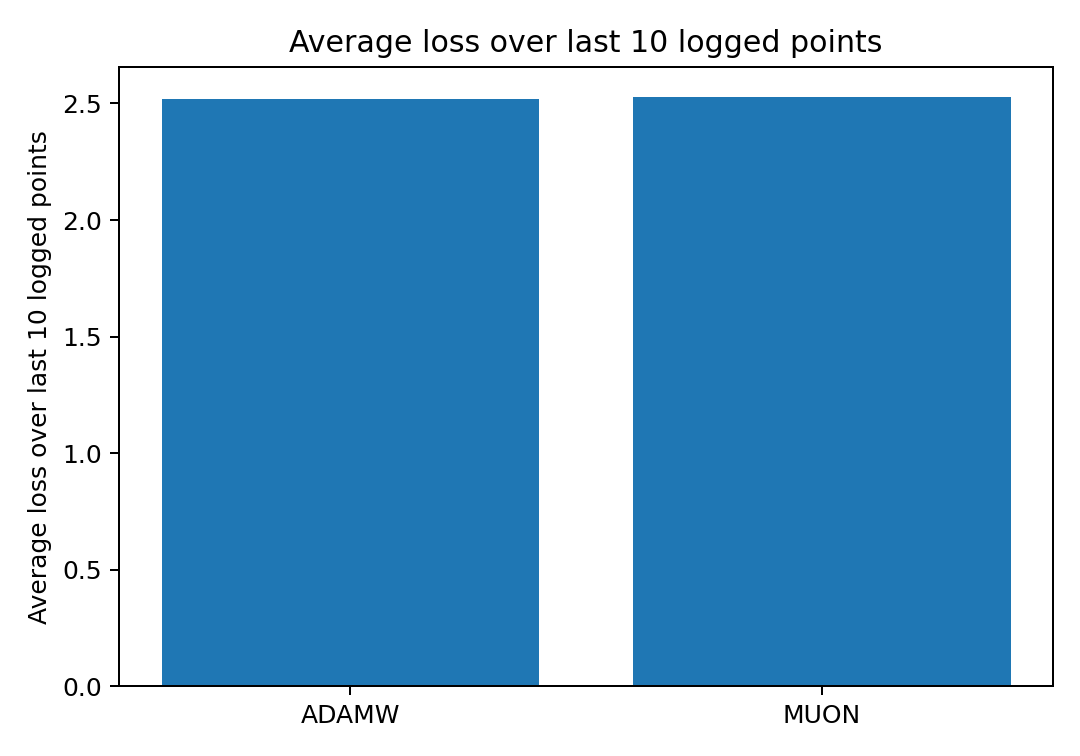
\includegraphics[width=0.58\textwidth]{figures/best_tail_loss_comparison.png}
    \caption{Average loss over the last 10 logged points for the best matched runs.}
    \label{fig:best-loss}
\end{figure}

\subsection{PIQA evaluation}
PIQA results are shown in Table~\ref{tab:piqa} and Figure~\ref{fig:piqa}.
The unfine-tuned base model achieved the highest PIQA accuracy in this comparison.
Both fine-tuned models obtained nearly identical PIQA scores, and both were slightly lower than the base model.
This indicates that short generic-text fine-tuning on OpenWebText does not meaningfully improve PIQA in this setup.

\begin{table}[H]
\centering
\caption{PIQA evaluation results.}
\label{tab:piqa}
\begin{tabular}{lrr}
\toprule
Model & Accuracy & Std. error \\
\midrule
Base Qwen2.5-0.5B & 0.7051 & 0.0106 \\
AdamW fine-tuned & 0.6997 & 0.0107 \\
Muon fine-tuned & 0.6997 & 0.0107 \\
\bottomrule
\end{tabular}
\end{table}

\begin{figure}[H]
    \centering
    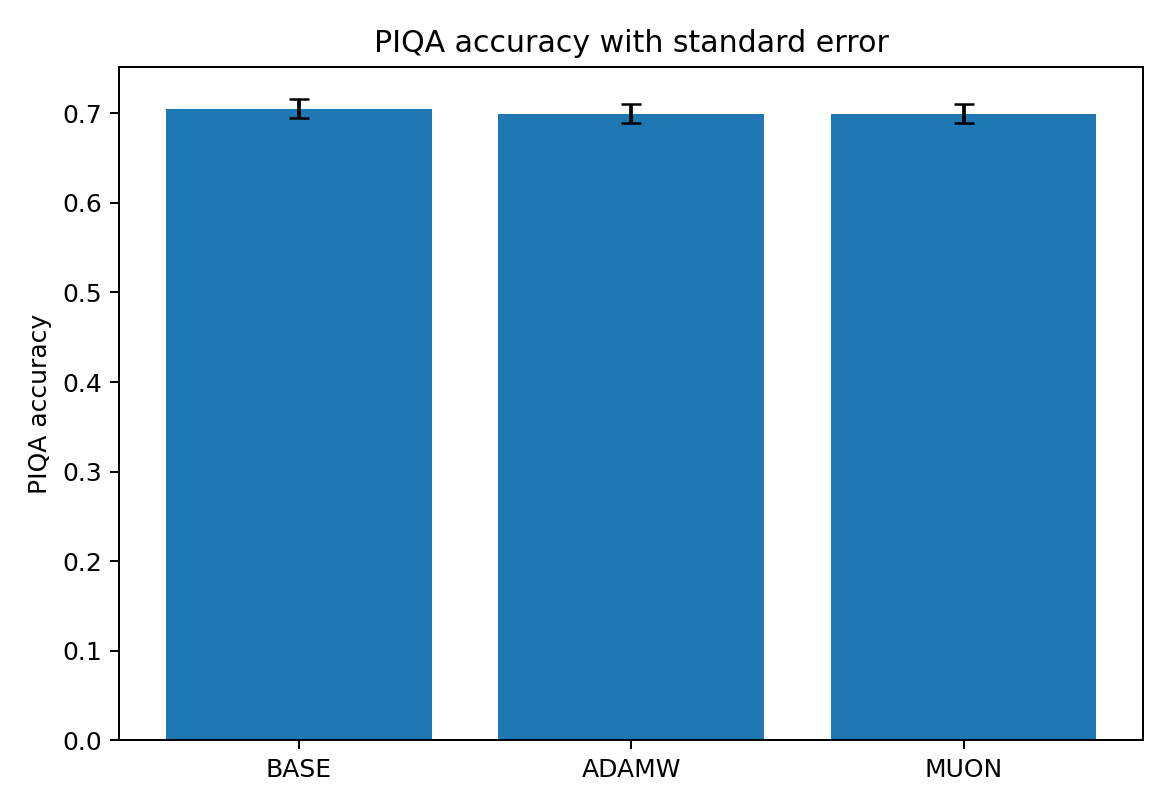
\includegraphics[width=0.62\textwidth]{figures/piqa_accuracy.png}
    \caption{PIQA accuracy with standard error bars.}
    \label{fig:piqa}
\end{figure}

\section{Discussion}
The main practical result is that AdamW was the better optimizer for this specific LoRA fine-tuning regime.
Its training loss was marginally lower, its total runtime was substantially lower, and its peak memory usage was indistinguishable from Muon's.

The likely reason is the trainable-parameter regime.
Muon is designed around orthogonalized updates for matrix-like parameters, and this can be attractive when large dense hidden weights are trained.
In the present setup, however, only a relatively small set of low-rank LoRA matrices is trainable.
As a result, the orthogonalization step introduces noticeable optimizer overhead without producing a compensating memory or convergence advantage.

The PIQA results reinforce a second point: the fine-tuning corpus and evaluation benchmark matter.
OpenWebText is a generic web-text corpus, while PIQA is a physical commonsense reasoning benchmark.
Under short fine-tuning with only 5,000 text samples, neither optimizer produced a measurable PIQA gain relative to the base model.
This suggests that the training objective improved adaptation to the training distribution more than it improved task-specific reasoning ability.

\section{Limitations}
This study has several limitations:
\begin{itemize}[leftmargin=1.5em]
    \item only one model size was tested
    \item only LoRA fine-tuning was considered, not full-model fine-tuning
    \item only one LoRA target pattern (\texttt{q\_proj}, \texttt{v\_proj}) was used
    \item the training corpus is generic web text, not PIQA-specific supervision
    \item challenge experiments (MeZO and a deliberate Muon+AdamW split with non-empty branches) were not included in the main comparison
\end{itemize}

\section{Conclusion}
For LoRA fine-tuning of Qwen2.5-0.5B on an RX 7900 XTX under a matched 5,000-sample, 2-epoch setup, AdamW and Muon achieved similar training losses, but AdamW was materially faster and used the same amount of peak memory.
PIQA evaluation showed no downstream advantage for either fine-tuned model over the base model in this experiment.
Therefore, within this specific low-rank adapter training regime, AdamW is the stronger practical baseline.

A natural next step is to test Muon in a denser trainable-parameter regime, such as partial or full-model fine-tuning, or to implement the challenge-mode hybrid split where distinct trainable parameter groups are intentionally assigned to Muon and AdamW.

\appendix
\section{Sweep summary}
Table~\ref{tab:sweep} lists all runs included in the learning-rate sweep.

\begin{center}
\small
\begin{longtable}{lrrrrr}
\caption{Learning-rate sweep summary.} \label{tab:sweep}\\
\toprule
Run & LR & Time (s) & Peak mem (GB) & Final loss & Avg. last 10 \\
\midrule
\endfirsthead
\toprule
Run & LR & Time (s) & Peak mem (GB) & Final loss & Avg. last 10 \\
\midrule
\endhead
adamw\_lora\_lr1e4 & 0.0001 & 318.07 & 7.546 & 2.515 & 2.538 \\
adamw\_lora\_lr3e4 & 0.0003 & 318.94 & 7.546 & 2.507 & 2.530 \\
adamw\_lora\_lr1e3 & 0.001 & 319.31 & 7.546 & 2.496 & 2.517 \\
adamw\_lora\_lr3e3 & 0.003 & 318.67 & 7.546 & 2.503 & 2.523 \\
muon\_lora\_lr3e4 & 0.0003 & 398.51 & 7.544 & 2.509 & 2.534 \\
muon\_lora\_lr1e3 & 0.001 & 398.84 & 7.544 & 2.503 & 2.529 \\
muon\_lora\_lr3e3 & 0.003 & 395.45 & 7.544 & 2.509 & 2.532 \\
muon\_lora\_lr1e2 & 0.01 & 398.45 & 7.544 & 6.141 & 6.073 \\

\bottomrule
\end{longtable}
\end{center}

\end{document}
